%\documentclass[
  bibliography=totoc,     % Literatur im Inhaltsverzeichnis
  captions=tableheading,  % Tabellenüberschriften
  titlepage=firstiscover, % Titelseite ist Deckblatt
]{scrartcl}

% Paket float verbessern
\usepackage{scrhack}

% Warnung, falls nochmal kompiliert werden muss
\usepackage[aux]{rerunfilecheck}

% unverzichtbare Mathe-Befehle
\usepackage{amsmath}
% viele Mathe-Symbole
\usepackage{amssymb}
% Erweiterungen für amsmath
\usepackage{mathtools}

% Fonteinstellungen
\usepackage{fontspec}
% Latin Modern Fonts werden automatisch geladen
% Alternativ zum Beispiel:
%\setromanfont{Libertinus Serif}
%\setsansfont{Libertinus Sans}
%\setmonofont{Libertinus Mono}

% Wenn man andere Schriftarten gesetzt hat,
% sollte man das Seiten-Layout neu berechnen lassen
\recalctypearea{}

% deutsche Spracheinstellungen
\usepackage[ngerman]{babel}


\usepackage[
  math-style=ISO,    % ┐
  bold-style=ISO,    % │
  sans-style=italic, % │ ISO-Standard folgen
  nabla=upright,     % │
  partial=upright,   % │
  mathrm=sym,        % ┘
  warnings-off={           % ┐
    mathtools-colon,       % │ unnötige Warnungen ausschalten
    mathtools-overbracket, % │
  },                       % ┘
]{unicode-math}

% traditionelle Fonts für Mathematik
\setmathfont{Latin Modern Math}
% Alternativ zum Beispiel:
%\setmathfont{Libertinus Math}

\setmathfont{XITS Math}[range={scr, bfscr}]
\setmathfont{XITS Math}[range={cal, bfcal}, StylisticSet=1]

% Zahlen und Einheiten
\usepackage[
  locale=DE,                   % deutsche Einstellungen
  separate-uncertainty=true,   % immer Unsicherheit mit \pm
  per-mode=symbol-or-fraction, % / in inline math, fraction in display math
]{siunitx}

% chemische Formeln
\usepackage[
  version=4,
  math-greek=default, % ┐ mit unicode-math zusammenarbeiten
  text-greek=default, % ┘
]{mhchem}

% richtige Anführungszeichen
\usepackage[autostyle]{csquotes}

% schöne Brüche im Text
\usepackage{xfrac}

% Standardplatzierung für Floats einstellen
\usepackage{float}
\floatplacement{figure}{htbp}
\floatplacement{table}{htbp}

% Floats innerhalb einer Section halten
\usepackage[
  section, % Floats innerhalb der Section halten
  below,   % unterhalb der Section aber auf der selben Seite ist ok
]{placeins}

% Seite drehen für breite Tabellen: landscape Umgebung
\usepackage{pdflscape}

% Captions schöner machen.
\usepackage[
  labelfont=bf,        % Tabelle x: Abbildung y: ist jetzt fett
  font=small,          % Schrift etwas kleiner als Dokument
  width=0.9\textwidth, % maximale Breite einer Caption schmaler
]{caption}
% subfigure, subtable, subref
\usepackage{subcaption}

% Grafiken können eingebunden werden
\usepackage{graphicx}

% schöne Tabellen
\usepackage{tabularray}
\UseTblrLibrary{booktabs, siunitx}

% Verbesserungen am Schriftbild
\usepackage{microtype}

% Literaturverzeichnis
\usepackage[
  backend=biber,
]{biblatex}
% Quellendatenbank
\addbibresource{lit.bib}
\addbibresource{programme.bib}

% Hyperlinks im Dokument
\usepackage[
  german,
  unicode,        % Unicode in PDF-Attributen erlauben
  pdfusetitle,    % Titel, Autoren und Datum als PDF-Attribute
  pdfcreator={},  % ┐ PDF-Attribute säubern
  pdfproducer={}, % ┘
]{hyperref}
% erweiterte Bookmarks im PDF
\usepackage{bookmark}

% Trennung von Wörtern mit Strichen
\usepackage[shortcuts]{extdash}

\author{%
  Vincent Wirsdörfer\\%
  \href{mailto:vincent.wirsdoerfer@udo.edu}{authorA@udo.edu}%
  \and%
  Joris Daus\\%
  \href{mailto:joris.daus@udo.edu}{authorB@udo.edu}%
}
\publishers{TU Dortmund – Fakultät Physik}


%\begin{document}
\section{Versuchsaufbau}

Die Funktionsweise des Michelson Interferometers beschränkt sich  im Wesentlichen auf die Reflexe und Interferenzen 
von Laserstrahlen. An einem teildurchlässigen Spiegel wird das kohärente Licht eines Diodenlasers partiell reflektiert 
und transmittiert. Dabei befindet sich der Spiegel in Winkel von \qty{45}{\degree} zur Propagationsrichtung des Laserstrahls.
Dies lässt sich anhand der untenstehenden Abbildung \ref{fig:Aufbau} nachvollziehen. Spiegel \uproman{1} dient zur Reflexion des 
am Spiegel reflektierten Teilstrahls des Lasers. Analog wird der transmittierte Teilstrahl an Spiegel \uproman{2} reflektiert.
Beide Strahlen laufen somit erneut zusammen und können miteinander interferieren. Auf einen Schirm im Strahlenweg oder mit einer
Photodiode kann das Interferenzmuster direkt visualisiert bzw. gezeigt werden.\\

\noindent Unter Zuhilfenahme eines Schmitt-Triggers wird das Signal der Photozelle in einen Impuls umgewandelt. Dieser bewirkt,
dass die analogen Signale der Photozelle verstärkt werden und bei Überschreiten eines gewissen Schwellwertes als digitale 1 von 
einem Zähler registriert werden. Die Spannungen der Photozelle unterhalb der Schwelle erzeugen im Gegensatz eine 0.\\

\noindent Die in der Abbildung erkennbare Gaszelle kann alternierend evakuiert und belüftet werden und dient zur Ermittlung 
von Brechungsindizes verschiedener Gase.

\begin{figure}[H]
    \centering
    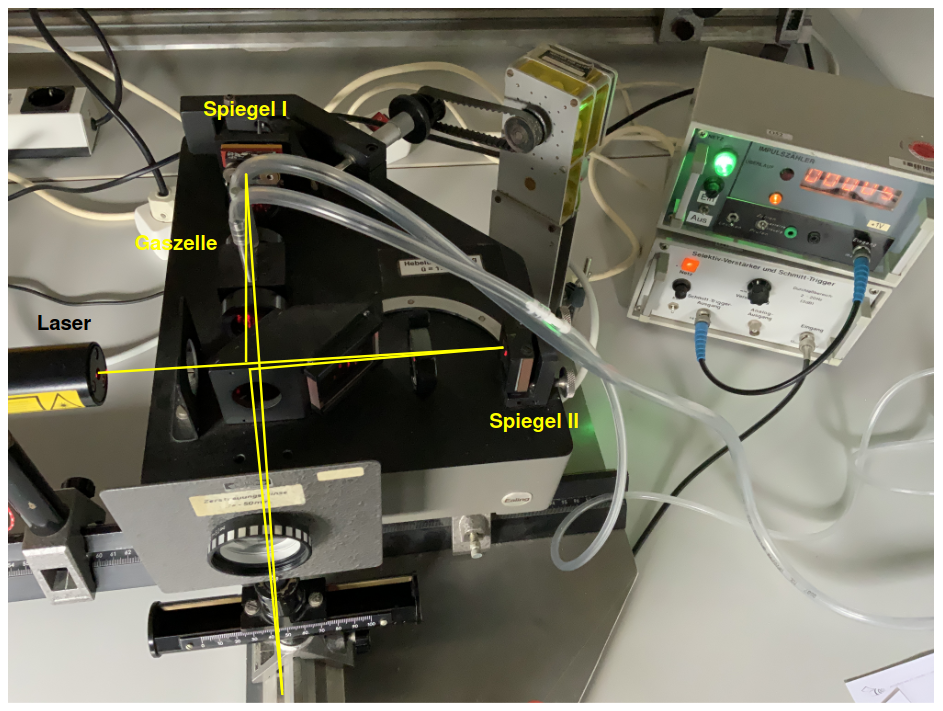
\includegraphics[height=5cm]{content/Aufbau.png}
    \caption{Versuchsaufbau des Michelson Interferometers\cite{Versuchsanleitung_v401}.}
    \label{fig:Aufbau}
\end{figure}

\section{Versuchsdurchführung}
\label{sec:Versuchsdurchfuehrung}

\subsection{Justage der Apparatur}

Zu Beginn des Experiments wird die Versuchsapparatur justiert. Hierzu werden die einzelnen Reflexe an allen Spiegel der Konstruktion 
untersucht. Mittels der Teilnehmerkarte werden die einzelnen Strahlengänge blockiert um die auf dem Schirm, welcher ebenfalls mit einer 
Teilnehmerkarte simuliert wird, beobachtbaren Laserstrahlen zu identifizieren. Somit kann festgestellt werden, welche Teilstrahlen der 
Reflexion und Transmission die Interferenzerscheinungen hervorrufen. Durch Verschieben des Spiegels \uproman{2} sowie Drehen des Lasers
selbst kann ein bestimmtes Interferenzmaximum in korrekte Position gebracht werden. Unter dieser Einstellung können nun die Messungen 
durchgeführt werden.

\subsection{Messung der Wellenlänge}

Die experimentelle Ermittlung der Wellenlänge besteht essenziell daraus, die Mikrometerschraube auf eine Einstellung von \qty{2}{\milli\meter}
zu bringen. Dies stellt sicher, dass die Schraube in einem Bewegungsradius von \qty{5}{\milli\meter} rotiert werden kann. Demzufolge wird so 
lange eine Messung durchgeführt, bis die Schraube \qty{7}{\milli\meter} erreicht. Die zu diesem Zeitpunkt angezeigte Zählrate wird notiert.
Im Anschluss wird die gleiche Messung im Bereich von \qty{7}{\milli\meter} bis \qty{2}{\milli\meter} ausgeführt. Dieser Prozess wird insgesamt 
fünfmal wiederholt, sodass zehn Zählraten ausgewertet werden können.

\subsection{Brechungsindex von Luft}

Die Bestimmung des Brechungsindex von Luft beruht auf einem ähnlichen Prinzip wie die vorherige Teilaufgabe. Mit einer Pumpe wird die Gaszelle 
der Apparatur abwechselnd evakuiert und belüftet. Beim Evakuieren wird der Luftdruck der Gaszelle auf \qty{500}{\milli \meter Hg} verringert.
In diesem Fall misst der Zähler die Anzahl der Interferenzmaxima. Hierbei wird versucht, 
für Evakuierung und Belüftung eine in etwa identische Zeit zu erreichen. Insgesamt werden je fünf Zählraten für den Evakuierungs- und 
Lüftungsprozess aufgenommen. Zusätzlich wird für die Berechnung des Index die Raumtemperatur sowie der Normaldruck gemessen. 

\section{Messwerte}

Zur Bestimmung der Wellenlängen werden die Anzahl der gezählten Maxima gemessen, wenn sich der Spiegel um \qty{5}{\milli \meter} bewegt. 
Dabei ergeben sich die folgenden Messwerte:



\begin{table}[H]
    \caption{Anzahl der Interferenzmaxima und Minima zur Bestimmung der Wellenlänge.}
    \label{tab:Wellenlaenge}
    \begin{minipage}[t]{0.5\textwidth}
        \vspace{0pt}
        \centering
    \begin{tblr}{
        colspec = {S S},
        row{1} = {guard, mode = math},
        }
        \toprule
            \text{Messung Nr.} & \text{Anzahl der Interferenzen} \\
        \midrule
            1   &   2999 \\
            2   &   3046 \\
            3   &   2698 \\
            4   &   3000 \\
            5   &   2990 \\
    \end{tblr}
\end{minipage} \hfill
\begin{minipage}[t]{0.5\textwidth}
        \vspace{0pt}
        \centering
    \begin{tblr}{
            colspec={S S},
            row{1} = {guard, mode = math},
        }
        \toprule
            \text{Messung Nr.} & \text{Anzahl der Interferenzen} \\
        \midrule
            6   &   2971 \\
            7   &   3006 \\
            8   &   2959 \\
            9   &   2991 \\
            10  &   2955 \\
        \end{tblr}
    \end{minipage}\hfill
\end{table}

\noindent Anschließend werden die Umgebungswerte für die Messung des Brechungsindex aufgenommen. Die Raumtemperatur wird über 
ein digitales Thermometer bestimmt und beträgt \qty{23.7\pm0.05}{\celsius}. Der Luftdruck wird mithilfe der Sportuhr Garmin 
Fenix 5 aufgenommen und beträgt $p_0=\qty{1010.0\pm0.05}{\milli\Bar}$. Wie bereits erwähnt, wird der Luftdruck in 
der Gaszelle auf \qty{500}{\milli \meter Hg} verringert, und währenddessen die Interferenzmaxima gezählt. Anschließend wird 
der Luftdruck wieder ausgeglichen und erneut die Maxima gezählt. So ergeben sich die folgenden Zählraten. 

\begin{table}[H]
    \caption{Anzahl der Interferenzmaxima und Minima zur Bestimmung des Brechungsindizes.}
    \label{tab:Wellenlaenge}
    \begin{minipage}[t]{0.5\textwidth}
        \vspace{0pt}
        \centering
    \begin{tblr}{
        colspec = {S S},
        row{1} = {guard, mode = math},
        }
        \toprule
            \text{Messung Nr.} & \text{Evakuierung} \\
        \midrule
            1   &   31   \\
            2   &   30   \\
            3   &   31   \\
            4   &   26   \\
            5   &   27   \\
    \end{tblr}
\end{minipage} \hfill
\begin{minipage}[t]{0.5\textwidth}
        \vspace{0pt}
        \centering
    \begin{tblr}{
            colspec={S S},
            row{1} = {guard, mode = math},
        }
        \toprule
            \text{Messung Nr.} & \text{Belüftung} \\
        \midrule
            6   &   27 \\
            7   &   27 \\
            8   &   26 \\
            9   &   26 \\
            10  &   27 \\
        \end{tblr}
    \end{minipage}\hfill
\end{table}




%\end{document}

